\documentclass[11pt]{article}

\usepackage[margin=1in]{geometry}
\usepackage{amsmath,amssymb}
\usepackage{booktabs}
\usepackage{graphicx}
\usepackage{hyperref}
\usepackage{url}
\usepackage{xcolor}

\hypersetup{
  colorlinks=true,
  linkcolor=blue,
  citecolor=blue,
  urlcolor=blue
}

\title{FANoS-v2: Feedback-Controlled Momentum with Thermostat Damping for Lightweight Neural Optimization}
\author{Nalin Dhiman\\FANoS-v2 Project}
\date{Draft v0.2 Evidence Report, May 2026}

\begin{document}
\maketitle

\begin{abstract}
We introduce FANoS-v2, a PyTorch optimizer that augments RMS-preconditioned momentum with a feedback controller over update energy. The optimizer stores momentum in parameter-update units, applies a non-negative thermostat damping coefficient, and exposes diagnostic quantities for stability auditing. We report a v0.2 empirical study on lightweight image-classification benchmarks, small scientific objectives, a single Poisson-1D PINN setting, and an EEGBCI smoke benchmark. The strongest current result is the experimental \texttt{FANoSV2Fast} configuration: on five-seed reduced-sample MNIST, Fashion-MNIST, and CIFAR-10 runs, it improves mean top-1 accuracy over AdamW by $0.889$, $2.197$, and $2.666$ percentage points, respectively. However, it remains $49.8\%$, $61.6\%$, and $56.8\%$ slower than AdamW on those same runs. The current evidence supports FANoS-v2 as a promising research optimizer with a repeated-seed lightweight-vision signal, but it does not support claims that FANoS-v2 is a universal optimizer or a drop-in AdamW replacement. We identify the next blocking task as optimizer-core speed engineering, especially a dense diagonal fast path using batched or foreach-style tensor operations.
\end{abstract}

\section{Claim Boundary}

This manuscript is intentionally conservative. The safe claim is:
\begin{quote}
FANoS-v2 is a feedback-controlled optimizer with repeated-seed accuracy gains on lightweight vision benchmarks and a plausible, but under-validated, scientific-objective direction.
\end{quote}
The unsafe claims are that FANoS-v2 is a universal AdamW replacement, that it is production-competitive on wall-clock time, or that it is broadly validated for physics-informed neural networks. The data below do not establish those stronger claims.

\section{Background and Motivation}

Adam and AdamW remain strong default optimizers for stochastic neural-network training \cite{kingma2014adam,loshchilov2017adamw}. Their appeal is not only empirical accuracy; it is also implementation efficiency, mature framework support, and predictable tuning. Any new optimizer must therefore beat a high bar: it must either improve accuracy at acceptable cost, reduce memory or communication cost, or solve a failure mode not handled by the defaults.

FANoS-v2 explores a different axis: instead of treating the momentum coefficient as fixed or manually scheduled, it introduces a feedback-controlled damping variable that responds to update energy. The design is loosely inspired by thermostat ideas in molecular dynamics \cite{nose1984unified,hoover1985canonical}, but the implementation is a first-order stochastic optimizer rather than a Hamiltonian simulator. The optimizer targets objectives where momentum can help but uncontrolled update energy can destabilize progress.

\section{Optimizer Definition}

Let $\theta_t$ denote parameters and $g_t = \nabla_\theta L(\theta_t)$ the gradient. FANoS-v2 maintains a second-moment state $s_t$, an update buffer $u_t$ in parameter units, and a scalar damping variable $\zeta_t$ per parameter group. The default diagonal-preconditioned update is
\begin{align}
s_t &= \beta_2 s_{t-1} + (1-\beta_2) g_t^2,\\
\hat{s}_t &= \frac{s_t}{1-\beta_2^t},\\
\tilde{g}_t &= \frac{g_t}{(\sqrt{\hat{s}_t}+\epsilon)^\alpha},\\
\rho_t &= \rho_{\max,t}\exp(-\eta_t \zeta_t),\\
u_{t+1} &= \rho_t u_t - \eta_t \tilde{g}_t,\\
\theta_{t+1} &= \theta_t + u_{t+1}.
\end{align}
Here $\eta_t$ is the effective learning rate, $\rho_{\max,t}$ is the base momentum after warmup, and $\alpha$ is the preconditioner power. The implementation also includes a paper-audit mode that stores a physical descent velocity $v_t$ and applies $\theta_{t+1}=\theta_t-\eta v_{t+1}$; the parameter-unit update is the public default because it makes learning-rate semantics match ordinary deep-learning optimizers.

\subsection{Thermostat Controller}

The feedback controller compares observed update energy with a target based on the proposed preconditioned step:
\begin{align}
K_t &= \operatorname{mean}(u_t^2),\\
K_t^\star &= c\operatorname{mean}((\eta_t\tilde{g}_t)^2)+\epsilon.
\end{align}
The controller updates an exponential moving average of $K_t$ and $K_t^\star$, then applies a clipped log-ratio correction:
\begin{align}
e_t &= \operatorname{clip}\left(
\log\frac{\operatorname{EMA}(K_t)+\epsilon}
{\operatorname{EMA}(K_t^\star)+\epsilon},
-e_{\max},e_{\max}
\right),\\
\zeta_{t+1} &=
\operatorname{clip}\left((1-\lambda)\zeta_t+\gamma e_t,\zeta_{\min},\zeta_{\max}\right).
\end{align}
The public default constrains $\zeta_t\geq 0$, so the controller damps excess update energy rather than injecting negative friction. This is a stability choice, not a theorem of optimality.

\subsection{Presets}

The exact reference optimizer, \texttt{FANoSV2}, keeps full diagnostics and conservative guardrails. The experimental \texttt{FANoSV2Fast} preset keeps the same core update but removes gradient-norm based adaptive learning rate and clipping, updates thermostat diagnostics every four steps, and disables diagnostic object creation by default. This fast preset is based on the v0.2 ablation results, where the vision accuracy signal survived after removing gradient-norm scalar synchronization.

\section{Implementation}

The implementation is in PyTorch \cite{paszke2019pytorch}. Each parameter stores an update buffer and, for the default diagonal preconditioner, one second-moment tensor. The optimizer supports:
\begin{itemize}
\item diagonal, factored, and no-preconditioner modes;
\item optional lower-precision state tensors;
\item bounded thermostat damping;
\item optional adaptive preconditioner power;
\item diagnostics for $\zeta_t$, $\rho_t$, update energy, target energy, gradient norm, clipping scale, and effective learning rate.
\end{itemize}

The important engineering limitation is that the current implementation is still Python-loop heavy. Even after removing gradient-norm synchronization, \texttt{FANoSV2Fast} remains materially slower than AdamW. This points to the next v0.3 task: a dense diagonal fast path using foreach-style update operations and fewer per-parameter conversions.

\section{Experimental Protocol}

\subsection{Vision Benchmarks}

We use MNIST \cite{lecun1998mnist}, Fashion-MNIST \cite{xiao2017fashion}, and CIFAR-10 \cite{krizhevsky2009cifar}. The v0.2 final fast validation uses five seeds, 10,000 training samples, 2,000 test samples, five epochs, and the repository's small CNN architecture. The comparison is AdamW versus \texttt{FANoSV2Fast}; both use the same data splits, model class, seed, batch size, and learning-rate default in the benchmark script. These are lightweight optimizer-signal experiments, not state-of-the-art vision benchmarks.

\subsection{Ablations}

We ran scalar-synchronization ablations by varying the gradient-norm refresh interval. An initial ``no-gradnorm'' experiment was invalid because the \texttt{auto} preset overrode an explicit request to disable adaptive learning rate. That bug was fixed, tests were added, and the final \texttt{FANoSV2Fast} default was revalidated after the fix. This sequence matters because it prevents over-crediting a result that still used hidden adaptive learning rate.

\subsection{Scientific and EEG Checks}

We include preliminary non-vision checks from the fixed full-study result root: Rosenbrock, noisy regression, ODE fitting, sequence memory, a single Poisson-1D PINN preset, and an EEGBCI cross-subject benchmark. These are not treated as conclusive physics or EEG claims. PINNs in particular require broader validation because optimizer behavior can depend strongly on residual scaling, boundary-condition weighting, collocation sampling, and post-training LBFGS polish \cite{raissi2019pinn}.

\section{Results}

\subsection{Final Fast Vision Results}

Table~\ref{tab:vision-fast} gives the final v0.2 validation for the \texttt{FANoSV2Fast} default. The fast preset improves mean top-1 accuracy on all three lightweight vision tasks, but it remains slower than AdamW.

\begin{table}[h]
\centering
\caption{Final five-seed reduced-sample vision validation. Top-1 values are percentages. Runtime is wall-clock seconds reported by the benchmark script.}
\label{tab:vision-fast}
\resizebox{\textwidth}{!}{\begin{tabular}{lrrrrrr}
\toprule
Dataset & AdamW top-1 & FANoSFast top-1 & $\Delta$ top-1 & AdamW s & FANoSFast s & $\Delta$ time \\
\midrule
MNIST & 96.19 $\pm$ 0.37 & 97.08 $\pm$ 0.49 & 0.89 pp & 2.83 & 4.23 & 49.8\% \\
Fashion-MNIST & 85.98 $\pm$ 1.50 & 88.17 $\pm$ 0.67 & 2.20 pp & 2.66 & 4.30 & 61.6\% \\
CIFAR-10 & 51.17 $\pm$ 0.93 & 53.84 $\pm$ 1.38 & 2.67 pp & 3.53 & 5.53 & 56.8\% \\
\bottomrule
\end{tabular}
}
\end{table}

\begin{figure}[h]
\centering
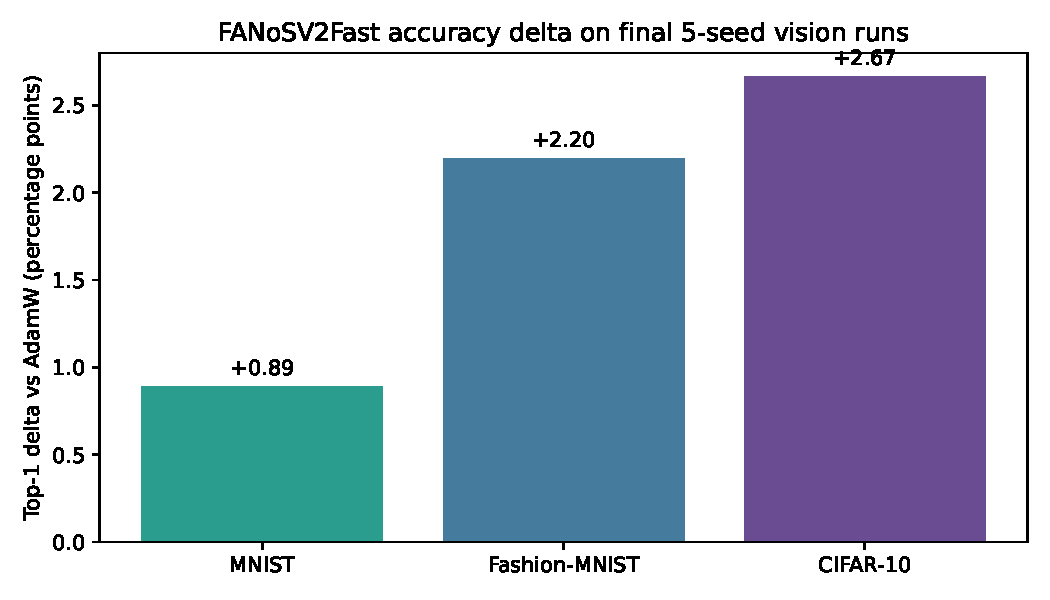
\includegraphics[width=0.82\textwidth]{figures/vision_accuracy_delta.pdf}
\caption{Top-1 accuracy delta of \texttt{FANoSV2Fast} relative to AdamW on final five-seed vision runs.}
\label{fig:vision-accuracy}
\end{figure}

\begin{figure}[h]
\centering
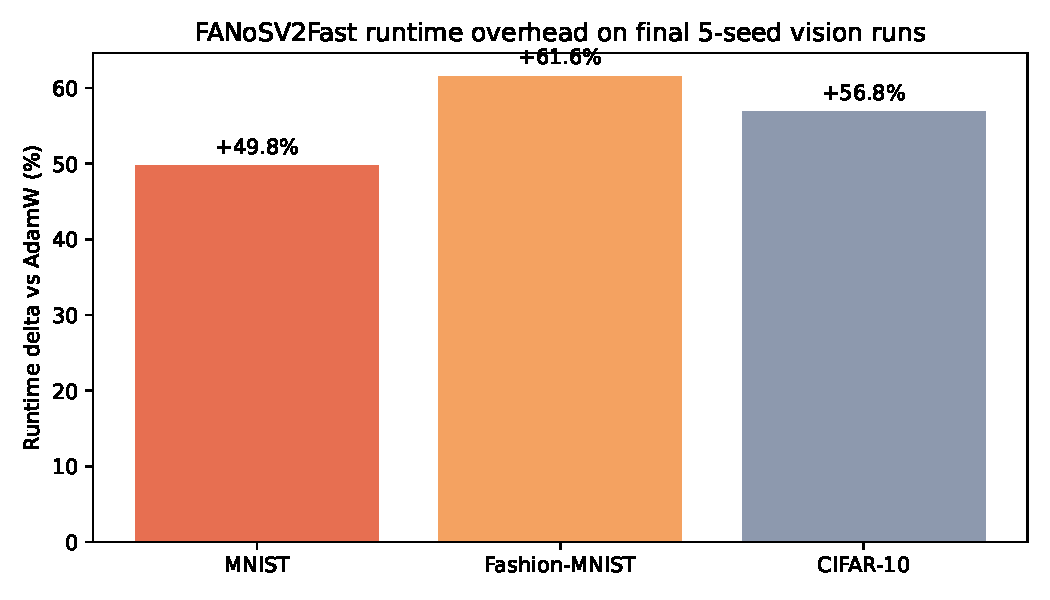
\includegraphics[width=0.82\textwidth]{figures/vision_runtime_delta.pdf}
\caption{Runtime overhead of \texttt{FANoSV2Fast} relative to AdamW on final five-seed vision runs. The overhead remains the central blocker for practical adoption.}
\label{fig:vision-runtime}
\end{figure}

\subsection{Gradient-Norm Synchronization Ablation}

The scalar-sync ablation initially suggested interval tuning could close the speed gap, but the result was not robust across datasets. The final useful finding was sharper: the vision accuracy signal survived removing both gradient clipping and adaptive learning rate from the fast preset. Table~\ref{tab:gradnorm} summarizes the interval sweep. It shows why interval tuning alone was not selected as the final v0.2 solution.

\begin{table}[h]
\centering
\caption{Gradient-norm refresh interval ablation. Values are five-seed summaries against the same AdamW baseline in each folder. The MNIST $k=4$ run was faster but had high variance; CIFAR-10 did not justify promotion.}
\label{tab:gradnorm}
\resizebox{\textwidth}{!}{\begin{tabular}{llrrrr}
\toprule
Dataset & Interval & FANoSFast top-1 & $\Delta$ top-1 & FANoSFast s & $\Delta$ time \\
\midrule
MNIST & 1 & 97.24 $\pm$ 0.37 & 1.04 pp & 5.62 & 89.5\% \\
MNIST & 2 & 96.85 $\pm$ 0.40 & 0.65 pp & 4.45 & 58.3\% \\
MNIST & 4 & 96.41 $\pm$ 1.22 & 0.21 pp & 3.86 & 42.3\% \\
MNIST & 8 & 96.66 $\pm$ 0.54 & 0.47 pp & 4.63 & 72.7\% \\
Fashion-MNIST & 2 & 87.20 $\pm$ 1.81 & 1.22 pp & 4.59 & 60.0\% \\
Fashion-MNIST & 4 & 87.24 $\pm$ 1.16 & 1.26 pp & 4.25 & 48.4\% \\
CIFAR-10 & 2 & 51.35 $\pm$ 2.01 & 0.18 pp & 5.96 & 65.3\% \\
CIFAR-10 & 4 & 51.10 $\pm$ 1.87 & -0.07 pp & 5.72 & 60.3\% \\
\bottomrule
\end{tabular}
}
\end{table}

\begin{figure}[h]
\centering
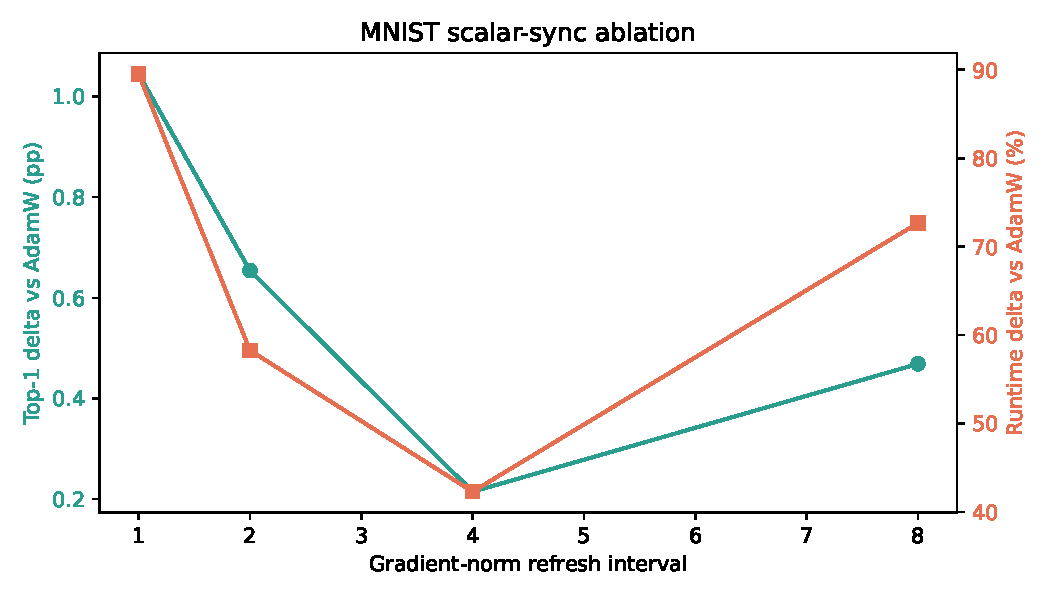
\includegraphics[width=0.82\textwidth]{figures/gradnorm_interval_ablation.pdf}
\caption{MNIST interval sweep. Higher intervals reduce some scalar synchronization but make the training behavior less predictable.}
\label{fig:gradnorm}
\end{figure}

\subsection{Preliminary PINN Result}

The single Poisson-1D PINN preset result is encouraging but narrow. The task-aware PINN configuration outperforms AdamW on the residual metric in this one setting, but it is slower and should not be generalized to physics problems broadly.

\begin{table}[h]
\centering
\caption{Preliminary Poisson-1D PINN preset result. Lower residual metric is better. This is a single task and does not establish broad PINN superiority.}
\label{tab:pinn}
\resizebox{0.78\textwidth}{!}{\begin{tabular}{lrrr}
\toprule
Optimizer & residual metric & loss & seconds \\
\midrule
fanosv2 & 6.472e-09 & 5.483e-04 & 9.69 \\
adamw & 1.863e-08 & 1.193e-03 & 3.11 \\
sgd & 5.142e-08 & 2.883e-03 & 2.58 \\
rmsprop & 2.278e-04 & 5.010e-03 & 3.07 \\
\bottomrule
\end{tabular}
}
\end{table}

\subsection{Preliminary EEG Result}

The fixed EEGBCI smoke benchmark no longer fails on MPS pooling, but the result is weak. FANoS auto has a small mean top-1 edge over AdamW with high variance and large time overhead. This is not enough for a strong EEG claim.

\begin{table}[h]
\centering
\caption{Preliminary EEGBCI five-seed result. This table is included to document the fixed benchmark, not to claim EEG superiority.}
\label{tab:eeg}
\resizebox{0.78\textwidth}{!}{\begin{tabular}{lrrr}
\toprule
Method & top-1 & $\Delta$ top-1 & $\Delta$ time \\
\midrule
FANoS auto & 45.33 $\pm$ 5.06 & 0.67 pp & 109.6\% \\
AdamW & 44.67 $\pm$ 4.47 & 0.00 pp & 0.0\% \\
\bottomrule
\end{tabular}
}
\end{table}

\subsection{Scientific Smoke Suite}

The small scientific suite is mixed. FANoS is competitive or useful on some tasks, but not uniformly better than AdamW or RMSProp. The ill-conditioned quadratic was a failure mode in the fixed full-study report and remains an explicit v0.3 target.

\begin{table}[h]
\centering
\caption{Selected scientific smoke results from the fixed full-study run. Lower metric is better except sequence-memory accuracy where higher is better. This is diagnostic evidence, not a broad scientific-ML benchmark.}
\label{tab:scientific}
\resizebox{\textwidth}{!}{\begin{tabular}{llrr}
\toprule
Task & Optimizer & metric & seconds \\
\midrule
rosenbrock100 & fanosv2 & 5.611e+00 & 2.05 \\
rosenbrock100 & adamw & 9.524e+00 & 0.52 \\
rosenbrock100 & rmsprop & 7.583e-01 & 0.51 \\
noisy\_small\_regression & fanosv2 & 5.714e-02 & 5.62 \\
noisy\_small\_regression & adamw & 5.318e-02 & 1.20 \\
noisy\_small\_regression & rmsprop & 6.056e-02 & 1.17 \\
ode\_exp\_fit & fanosv2 & 7.120e-03 & 1.85 \\
ode\_exp\_fit & adamw & 7.120e-03 & 0.40 \\
ode\_exp\_fit & rmsprop & 9.848e-03 & 0.39 \\
poisson\_pinn\_1d & fanosv2 & 1.445e-03 & 9.99 \\
poisson\_pinn\_1d & adamw & 1.863e-08 & 3.19 \\
poisson\_pinn\_1d & rmsprop & 2.278e-04 & 3.17 \\
sequence\_memory & fanosv2 & 1.000e+00 & 20.66 \\
sequence\_memory & adamw & 1.000e+00 & 11.99 \\
sequence\_memory & rmsprop & 7.266e-01 & 12.07 \\
\bottomrule
\end{tabular}
}
\end{table}

\section{Discussion}

The v0.2 result is meaningful but bounded. The repeated-seed lightweight-vision evidence survived a substantial simplification of the fast preset. This implies the observed accuracy gain is not merely an artifact of gradient clipping or adaptive learning-rate damping. The thermostat and feedback-momentum structure remain plausible contributors.

At the same time, the speed story is not solved. AdamW is highly optimized in PyTorch, while the current FANoS-v2 implementation performs more per-parameter Python work and more tensor operations. A release that presents FANoS-v2 as production-competitive would be misleading. The right framing is a research optimizer with an encouraging accuracy signal and a clear engineering bottleneck.

The physics story is even less mature. A single Poisson-1D PINN result supports a hypothesis that softer preconditioning and thermostat damping may help residual-heavy objectives. It does not prove general PINN or physics advantage. A credible physics follow-up should include heat, Burgers, and Poisson tasks, AdamW+LBFGS baselines, validation-grid error, residual terms, runtime, and failure rate.

\section{Limitations}

\begin{itemize}
\item The final vision validation uses small CNNs and reduced training subsets. It is not a ResNet-scale or transformer-scale benchmark.
\item Runtime remains $49.8\%$ to $61.6\%$ slower than AdamW in the final fast validation.
\item The implementation lacks a fused or foreach dense-diagonal fast path.
\item EEG and PINN evidence is preliminary and should not be marketed as solved.
\item Hyperparameter searches were pragmatic rather than exhaustive.
\item Statistical testing is limited to five seeds; confidence intervals should be expanded before a major claim.
\end{itemize}

\section{Release Recommendation}

For GitHub and PyPI, release FANoS-v2 as an alpha research optimizer. The README should lead with the conservative claim, document \texttt{FANoSV2} as the exact reference, and document \texttt{FANoSV2Fast} as the experimental speed preset. The next version should not add more small benchmark sweeps first; it should implement a dense-diagonal foreach fast path and then rerun the final three vision tasks.

\section{Conclusion}

FANoS-v2 reaches a credible v0.2 milestone: a reproducible optimizer implementation, a mathematically auditable update, a fast preset that preserves lightweight-vision accuracy gains, and clear evidence that runtime overhead remains the practical barrier. The optimizer is promising, but not finished. The strongest next step is engineering, not broader claims.

\begin{thebibliography}{10}

\bibitem{kingma2014adam}
Diederik P. Kingma and Jimmy Ba.
\newblock Adam: A Method for Stochastic Optimization.
\newblock arXiv:1412.6980, 2014.
\newblock \url{https://arxiv.org/abs/1412.6980}.

\bibitem{loshchilov2017adamw}
Ilya Loshchilov and Frank Hutter.
\newblock Decoupled Weight Decay Regularization.
\newblock arXiv:1711.05101, 2017; ICLR, 2019.
\newblock \url{https://arxiv.org/abs/1711.05101}.

\bibitem{lecun1998mnist}
Yann LeCun, Leon Bottou, Yoshua Bengio, and Patrick Haffner.
\newblock Gradient-Based Learning Applied to Document Recognition.
\newblock Proceedings of the IEEE, 86(11):2278--2324, 1998.

\bibitem{xiao2017fashion}
Han Xiao, Kashif Rasul, and Roland Vollgraf.
\newblock Fashion-MNIST: a Novel Image Dataset for Benchmarking Machine Learning Algorithms.
\newblock arXiv:1708.07747, 2017.
\newblock \url{https://arxiv.org/abs/1708.07747}.

\bibitem{krizhevsky2009cifar}
Alex Krizhevsky.
\newblock Learning Multiple Layers of Features from Tiny Images.
\newblock Technical report, University of Toronto, 2009.

\bibitem{paszke2019pytorch}
Adam Paszke et al.
\newblock PyTorch: An Imperative Style, High-Performance Deep Learning Library.
\newblock Advances in Neural Information Processing Systems 32, 2019.
\newblock \url{https://papers.neurips.cc/paper/9015-pytorch-an-imperative}.

\bibitem{raissi2019pinn}
Maziar Raissi, Paris Perdikaris, and George Em Karniadakis.
\newblock Physics-Informed Neural Networks: A Deep Learning Framework for Solving Forward and Inverse Problems Involving Nonlinear Partial Differential Equations.
\newblock Journal of Computational Physics, 378:686--707, 2019.
\newblock \url{https://doi.org/10.1016/j.jcp.2018.10.045}.

\bibitem{nose1984unified}
Shuichi Nose.
\newblock A Unified Formulation of the Constant Temperature Molecular Dynamics Methods.
\newblock Journal of Chemical Physics, 81:511--519, 1984.

\bibitem{hoover1985canonical}
William G. Hoover.
\newblock Canonical Dynamics: Equilibrium Phase-Space Distributions.
\newblock Physical Review A, 31(3):1695--1697, 1985.

\end{thebibliography}

\end{document}
